\documentclass{article} % For LaTeX2e
\usepackage{nips12submit_e,times, color}
\usepackage{natbib}
\usepackage[pdftex]{graphicx}
%\documentstyle[nips12submit_09,times,art10]{article} % For LaTeX 2.09


\title{Binary Separation on Heterogeneous Image}

\author{
Fisher Yu \\
\texttt{fy@princeton.edu}
\And
Nanxi Kang \\
\texttt{nkang@princeton.edu} 
\And
Siyu Liu\\
\texttt{siyuliu@princeton.edu}
}

\newcommand{\fix}{\marginpar{FIX}}
\newcommand{\new}{\marginpar{NEW}}

\nipsfinalcopy % Uncomment for camera-ready version

\begin{document}

\maketitle

test citation~\citep{Boykov2006graph}

\section{Introduction}
{\color{red} General description here}
\subsection{Motivation}
\subsection{Data}
We got our data from Google street view team and preprocessed it for
use in our project. The data was collected by a car equiped
with 8 cameras and 3 laser scanners. Each of the laser scanner can
scan a 180 degree 2D plane at each time. Two of the laser scanners
scanned vertically and the third one scanned horizontally. As the car moved, the car
positions were recorded by global positioning system. Those positions
were adjusted by the scans of the horizontal laser scanner using SLAM
(Simultaneous localization and mapping) techniques to get the best
precision. The 3D position of each laser scan point can be
estimated based on the relative positions of the car and laser
scanners and therefore a 3D point cloud can be built from the scans of
the vertical laser scanners. At the same time, the eight
cameras were taking pictures as the car moved. Although the cameras
were well calibrated, the images were taken by rolling shutters and
there could exist errors in terms of image projection model if we assume each
image were taken in a pinhole model.

Given the 3D point cloud and images, we project the points onto the
images with the estimated point positions, camera poses and projection
matrices. Then we can get images like Figure~\ref{fig-data_image}.

\begin{figure}[h]
\begin{center}
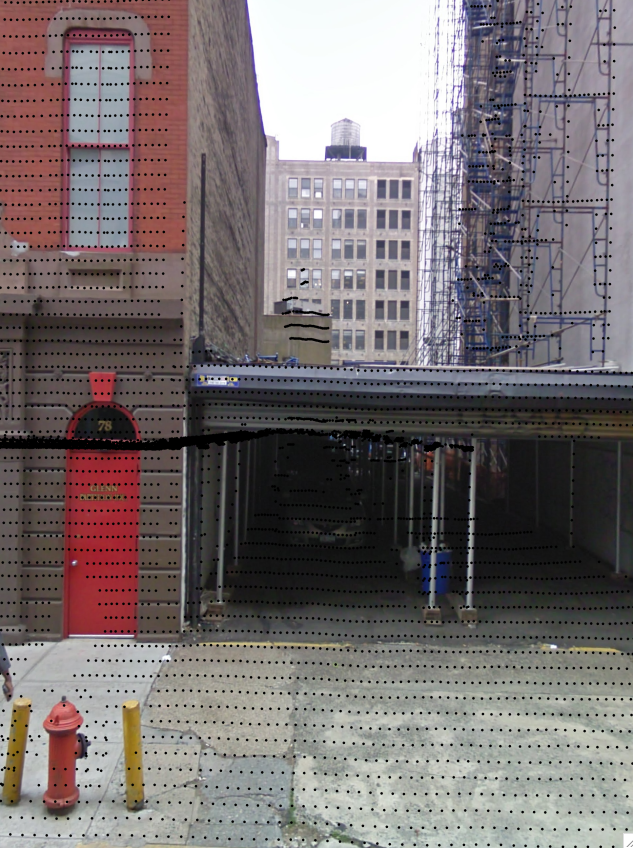
\includegraphics[height=0.5\linewidth]{./fig/image_sample.png}
\end{center}
\caption{An image with 3D points projected into it.}
\label{fig-data_image}
\end{figure}

In Figure~\ref{fig-data_image}, the black dots are the projections of
the 3D points on this image. As we can see, due to all kinds of possible
errors mentioned above, the 3D projections and the images are not well
aligned and we can't segment the images directly based on the depth of
the 3D scan points. In this project, we want to find the contour
between the background (the sky area) and foreground (all the objects
appears in the image, including roads and buildings). The models and
computing issue will be discussed in the methods section.

\section{Related Work}
As a common problem in vision, segmentation has been well studied in the past. There is a large literature on segmentation and clustering among which two main lines of methods are proposed previously, feature space clustering (e.g.~\citep{Comaniciu1997featurespace},~\citep{Comaniciu1999meanshift}) and graph-based approach (e.g.~\citep{Shi1997normalizedcuts},~\citep{Wu1993optimalgraph}). 

In feature sapce clustering, local features, such as low pass filter response, SIFT~\citep{Lowe2004sift}, etc., are firstly extracted from the given image. For color images, color information is often included. Then those features are concatenated to form a vector as a descriptor for each pixel. In order to segment the image, we might seek a clustering of feature vectors observed in the image. A compact region of image with distinct feature would be expected to have a corresponding high density area in the feature space. 

A natural approach is to model the observed feature vector using a Gaussian mixture model (GMM)~\citep{Carson2002bolbworld}. For a pre-determined number of clusters \textit{K}, the parameters can be fitted by Maximum Likelihood using EM algorithm. In addition, \textit{K} can be chosen using penalized likelihood (a.k.a. minimum description length), Baysian information criterion (BIC) and other model selection mechanisms. In addition, other variations are proposed by replacing GMM with K-means or low dimensional representation of the covariance matrix via matrix factorization. On the other hand, to avoid extra step of determining the number of clusters for the methods mentioned above, a non-parametric model based on kernel density estimation is proposed as an alternative. Mean-shift segmentation algorithm~\citep{Comaniciu2002robustapproach} considers the probability density of feature vectors obtained from a given image. An iterative update on the mean-shift equation is used to find the segmentation labels. 

Another branch of image segmentation algorithms is graph-based method. Instead of consider each pixel independently, we form a graph with each vertex representing an individual pixel and assign weights to edges according to some similarity measure. Then, the segments are determined by graph cuts.

One naive approach would be to calcualte connected components. We could use algorithms like Kruskal or Prime to simple remove edges between dissimilar pixels. However, this method is not robust to stray links. Thus,~\citep{Felzenszwalb2004Efficient} introduced an improved version of Kruskal algorithm which takes in account the local variantion within each component. An alternative proposal is to formulate segmentation as a max-flow/min-cut problem. One typical example of S-T Min Cut algorithms is the normalized cut introduced by~\citep{Shi2000Normalized}. This method takes into account the partition size of each segment so as to avoid tiny regions. In a more sophesticated setting, Markov Random Field (MRF), which we chosed for this project, is often used to combine probabilistic modeling and graph cut in order to provide better result. The goal of learning MRFs is to minimize the objective function (a.k.a. the energy function) which describes both fitness and connectivity among neighborhood. Several training algorithms have been proposed over the years, Iterated Conditional Modes (ICM)~\citep{Besag1986statisticalanalysis} uses "greedy" strategy to find local minimum; Graph Cuts, two most popular ones, swap-move and expansion-move were introduced in~\citep{Boykov2001Fast}; Max-Product Loopy Belif Propagation (LBP)~\citep{Felzenszwalb2004Efficient} and~\citep{Freeman2000lowlevel}, a variant algorithm from the original belif propagation supporting loops in the graph; Tree-reweighted Message Passing desbribed in~\citep{Kolmogorov2006messagepassing}.

\section{Methods}
Based on the previous work, we merge several ideas in our
project. First, to classify a pixel, we can first train a Gaussian
mixture model to summarize the variation of pixels in the background
and foreground separately. In another way to see this, we are getting
an approximate distance from a certain pixel value to the cluster it
belongs to and therefore we can get a cost to assign a certain pixel
to the foreground or background. On the other hand, in the Gaussian
mixture model, we are assigning an latent variable to each pixel. Due
to the isolation between adjacent pixels in the Gaussian model, it is
easy to imagine that the output of the binary classification will be
very noisy in the sense that the adjacent pixels will have different
labels although they have similar colors and belong to the same object
visually. To solve this problem, we use Markov random field(MRF) model to
constraint the relation between the labels of adjacent pixels. Also,
we use conditional random field(CRF) model to adapt this relation to
the difference of the pixel colors and therefore the model becomes
more flexible. Also, we explore various ways to utilize our laser
data. In the following subsections, we will discuss parts of our model
and elaborate how we use the scan data.
\subsection{Gaussian Mixture Model}
\subsection{Conditional Random Field}
\subsection{Inference}
\subsection{Use of Scan Data}
\section{Experiment}
The first experiment is done using GrabCut. As mentioned in previous section, we only use the distance transform image derived from laser point projections as an initialization for MRF in this case. The distance transform image is thresholded to form an initial labeling strategy for foreground and background. As a result, the extra information provided is not used across iterations. The result is shown in figure []. 

Note that since we assigned equal cost to edges across the image, cars having similar color as the sky would be segmented as the background.

Having observed this drawback, we decided to vary the cut cost according to our initial estimation of the segments. Note that, assuming foreground objects got scanned more often than background, the natural boundaries would occur at the transition between dense and sparse areas of projected LiDAR points. Thus, in the second experiment, LaserCut, we prepross the distance transform by running simple edge detection algorithm (i.e. Sobel operator) to extract possible boundaries between foreground and background. Therefore, for regions within the potential boundaries, some color differences would be tolerated by assigning smaller weights before the corresponding term in the energy funciton. In contrast, for pixels close to potential boundaries, we intend to rely more on color differences via larger weights to refine the boundary curve. The result is shown in figure [].

Comparing to GrabCut model, we successfully eliminated the white cars in the front from the background.

To further evaluate our model, we did another experiment on the same image with a widely used MRF model, Ising model. In this setting, color difference between neighboring pixels is completely ignored by assigning the same cost for connectivity to all edges in the MRF graph. The result is shown in figure [].

Taking a close look at the boundary Ising model found, we observed that the foreground objects are outlined by a "margin" of the sky. This is probably due to we only used Gaussian mixture model to measure the clustering in color. Since there are white cars on the road, the GMM would intend to label part of the sky as the foreground due to larger threshold on distance transform image. However, smaller threshold values would result in labeling the white cars in the front to background initial, which would be generally hard to correct in later iteration under this model.

\section{Evaluation}

In general, evaluating segmentation result is hard due to the absence of precise quantitative measurement without ground truth. In addition, there is another important issue centers around the use of energy to compare energy minimization algorithms. The goal in computer vision is not to compute the lowest energy but the most accurate one, besides computing the global minimum was shown to be NP-complete in general~\citep{Boykov2001Fast}. In the paper by~\citep{Szeliski2008Comparative}, a quantitative comparison between lowest energy achieved by different energy minimization algorithms and the energy calculated from ground truth provides experimental proof for this argument. Although one can argue that we could manually draw the boundaries for each image we used in this project, due to high resolution (1936 x 2592) and limited size of sample labling from different users we can account for given the time, the accuracy and unbiasness of the ground truth cannot be guaranteed.

As an alternative, we decided to conduct a comparison study among the three experiments we did mentioned in previous section. The best model as well as the final model we have is LaserCut which has the advantage of adaptiveness of initial guess through out all iterations. As we discussed before, comparing to GrabCut model, LaserCut successfully classified the cars with similar color as the background as part of the foreground. This observation suggests the effectiveness of adaptively using extra information acquired from LiDAR scan. On the other hand, comparing to Ising model, LaserCut could provide more complicated and accurate boundary between foreground and background, which indicates the effectiveness of separation on color differences when close to the boundary.

Granted, there are still areas near the boundary being mislabelled, for instance, some leaves of the tree in figure []. It is generally hard to determine the exact bounday of such complicated foreground object. Even when we have captured images with such high resolution, it is still far from certain that all the details of objects far back to the scene can be accurately preserved. Moreover, even though we can somehow manage to obtain all the details in the scene, the correctness of boundaries around complicated objects like trees would be rather subjective to different people.

Therefore, in spite of the fact that most of the model evaluation is based on visual check in this project, we hope our observations and analysis could make a plausible case for the advantage of LaserCut model over the others.

\section{Conclusion}

\bibliography{final}
\bibliographystyle{abbrvnat}


\end{document}
